\subsection{Theory}

The entropy is calculated for all components.
If a single decision can give information about a class or the removal of a class it is considered to be a high information gain.
Thus such a decision must be taken at the root of the tree.
Since the train data provided to the tree is only a subset of all the data the tree will classify, as it is with random inputs such as handwriting, every split carries a certain confidence in its classification.

\begin{figure}[h]
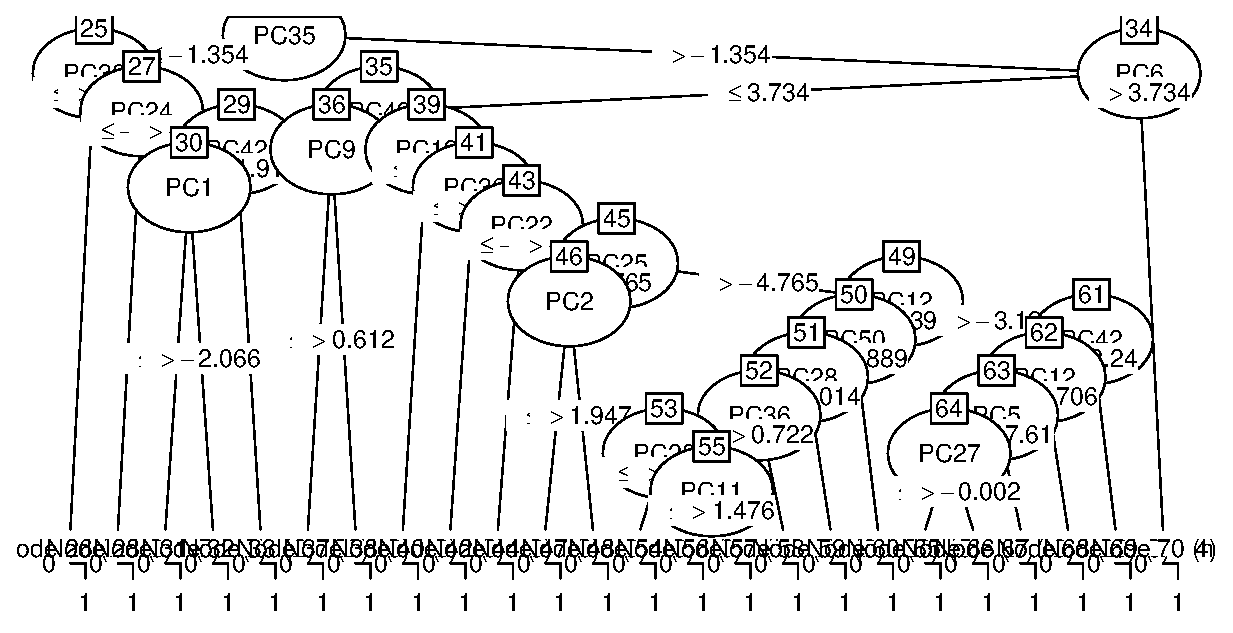
\includegraphics[width = \textwidth]{graphics/tree_section}
\caption[Visualization of a tree.]{Visualization of a small section of the tree.}
\label{fig:tree_section}
\end{figure}

Building a tree can be done using the ``C50'' library in R.
% The tree with the training data of 15 people (56000 cases) contains 6338 nodes.
A small section of the tree is shown in figure \ref{fig:tree_section}.
Each node shows which principal component and the split to which the decision is made.
Each leaf shows the probability of a classification.
The leftmost leaf (node 20) has n=2. This means that there are 2 cases where the decision splitting leads down to this node.
Both nodes are of class 10 so there is 100\% confidence that the number is of class 10.
On the right there is 65 cases in which the result is of class 1. 
This is a better indicator as it does not appear to be an random error in the data set.
The rightmost node has 4 results of the training data and cannot give a clear picture.
One is of class 4, one of 8 and two of class 10. 
When training this data half of the numbers will be misclassified.

A way to improve the decision tree is to remove nodes which is deemed to not be of significance.
This is called pruning, borrowing the vocabulary of gardening.
There are several ways to prune a tree.
The ``C5.0'' function can prune by increasing the confidence factor. 
The default is 25\% and thus the leaf node 22 in figure \ref{fig:tree_section} with 1/4 confidence is kept.
If the confidence of a node would fall below the confidence factor used for pruning, the leaf would be converted into a node with two leafs.
This will make it possible to make better decisions based on the data input to the tree.
\todo[inline]{changed the line above, so check it, and make the line below clearer. Isn't what you call a node a leaf and vice versa? 
Do you mean that the second way is to increase the number of "leafs" connected to the node such that you have two or more threshold for the data? 
Such that you have say x < 0.5, 0.5 < y < 1, 1 < z where z, y and z are the new nodes? }
Another pruning option is to increase the minimum number of nodes in a leaf. 
This will remove the noise created by a few selection of digits which creates a new split.
The default minimum number of nodes is 2.
Having this number too high will cause the confidence to go down as digits are lumped together. 